\section{Nurul Izza Hamka - 1174062}
\subsection{Teori}
\begin{enumerate}

\item Jelaskan kenapa kata-kata harus dilakukan vektorisasi, dilengkapi dengan ilustrasi atau gambar.

Vektorisasi pada kata-kata harus dilakukan karna dengan dilakukannya vektorisasi kita
dapat mengetahui berapa banyak jumlah kata yang muncul disetiap kalimat. Vektorisasi
ini juga bertujuan untuk menentukan kata keywords atau kata kunci yang nantinya
memudahkan pembaca dalam mencari kata atau kalimat yang dicari.

\begin{figure}
	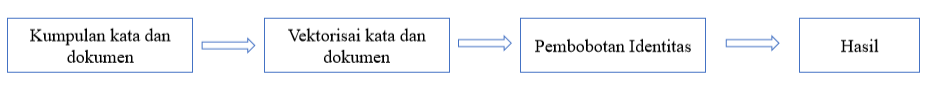
\includegraphics[width=4cm]{figures/1174062/5/teori1.png}
	\centering
	\caption{Vektorisasi Kata}
\end{figure}

\item Jelaskan mengapa dimensi dari vektor dataset google bisa sampai 300, dilengkapi dengan ilustrasi atau gambar.

Karena setiap objek memiliki identitas khusus, misalnya dalam dataset Google ini
memiliki 3 objek, kucing, anjing, dan ayam yang disetujui. Kemudian dari masingmasing objek dibandingkan dataset antara kucing dan anjing kemudian kucing dan
ayam. Hasil yang diperoleh untuk kucing dan anjing sekitar 75persen sedangkan untuk
kucing dan ayam yang memiliki persentase 15persen.

\begin{figure}
	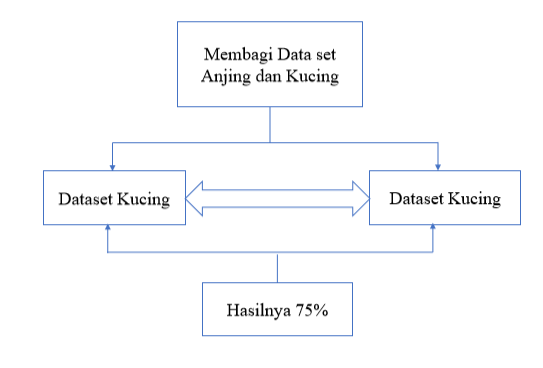
\includegraphics[width=4cm]{figures/1174062/5/teori2.png}
	\centering
	\caption{Dimensi Vektor}
\end{figure}

\item Jelaskan konsep vektorisasi untuk kata, dilengkapi dengan ilustrasi atau gambar

Konsep untuk vektorisasi kata sama dengan masukan atau input pada kata-kata di mesin
pencari. Maka anggaplah itu akan dikeluarkan sebagai saran tentang kata tersebut. Jadi
kata data diperoleh dari hasil yang diolah dalam kalimat sebelumnya yang telah
diproses. \\
Contoh sederhana dalam kalimat berikut (Silakan berlangganan saluran saya,
terima kasih teman), dalam kalimat itu terkait dengan kalimat saluran, kata akan dibuat
data pelatihan untuk mesin. Jadi kita kompilasi kata channel, maka mesin akan
menampilkan hubungannya dengan kata tersebut.

\item Jelaskan konsep vektorisasi untuk dokumen, dilengkapi dengan ilustrasi atau gambar.

Dokumen bukanlah data terstruktur karena jauh dari bentuk tabel (baris dan kolom).
Perlu metodologi pembentukan suatu data terstruktur untuk mewakili dokumen.
Langkah awal adalah harus menentukan features yang mewakiliki seluruh kumpulan
dokumen.\\
Sama halnya dengan vektorisasi kata, yang membedakan hanya pada proses awalnya.
Untuk vektorisasi dokumen ini, mesin akan membaca semua kalimat yang terdapat
pada dokumen tersebut, lalu kalimat yang terdapat pada dokumen akan di pecah
menjadi kata-kata.

\item Jelaskan apa mean dan standar devisiasi, dilengkapi dengan ilustrasi atau gambar.

Mean adalah perhitungan nilai rata-rata dari data yang ada. Nilai mean ini dapat kita
ambil dari hasil membagi jumlah data dengan banyaknya data yang ada.\\
Sedangkan standar deviasi adalah salah satu pengukuran statistika yang digunakan
untuk menjelaskan bagaimana sebaran data dalam sampel, dan seberapa dekat titik data
individu ke rata-rata nilai sampel.

\begin{figure}
	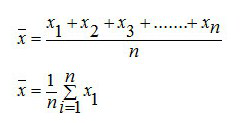
\includegraphics[width=4cm]{figures/1174062/5/teori51.png}
	\centering
	\caption{Rumus Mean}
\end{figure}


\begin{figure}
	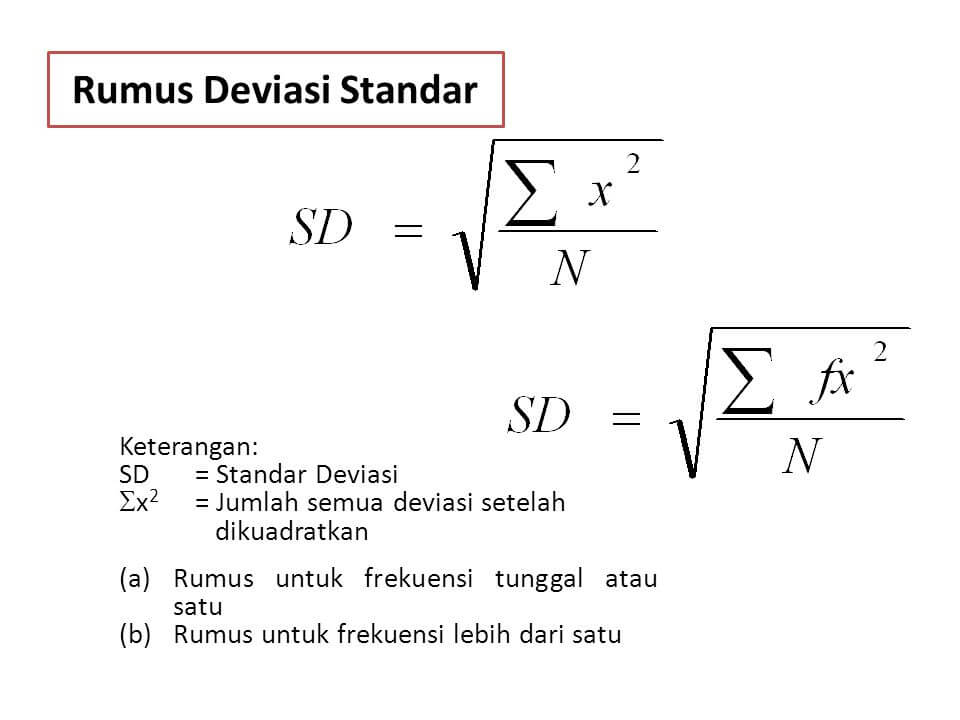
\includegraphics[width=4cm]{figures/1174062/5/teori52.png}
	\centering
	\caption{Standar Devisiasi}
\end{figure}

\item Jelaskan apa itu skip-gram, dilengkapi dengan ilustrasi atau gambar.

Skip-gram adalah salah satu teknik pembelajaran unsupervised-learning yang
digunakan untuk menemukan kata yang paling terkait untuk kata yang diberikan. Skipgram digunakan untuk memprediksi kata konteks untuk kata target yang diberikan. Ini
kebalikan dari algoritma CBOW. Di sini, kata target adalah input sedangkan kata
konteks adalah output. 

\begin{figure}
	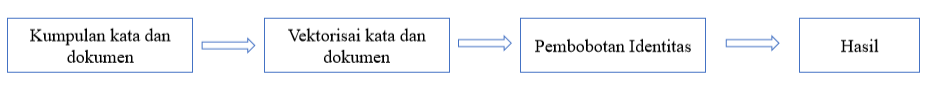
\includegraphics[width=4cm]{figures/1174062/5/teori1.png}
	\centering
	\caption{Skip-Gram}
\end{figure}
\end{enumerate}

\subsection{Praktek Program}
\begin{enumerate}

\item Cobalah dataset google, dan jelaskan vektor dari kata Love, faith, fall, sick, clear, shine, bag, car, wash, motor, cycle, dan cobalah untuk melakukan perbandingan  similitai dari masing-masing kata tersebut. Jelaskan arti outputan sinilirati dan setiap baris kode yang dibuat.

	\hfill\break
	\lstinputlisting[firstline=8, lastline=13]{src/1174062/5/1174062.py}

Kode diatas untuk malakukan import library gensim. Gensim ini untuk melakukan pemodelan dengan dataset atau topik yang sudah ditentukan.

	\hfill\break
	\lstinputlisting[firstline=14, lastline=46]{src/1174062/5/1174062.py}

\item Jelaskan dengan kata dan ilustrasi fungsi dari extract words dan PermuteSentences (harus beda dengan teman sekelas)

	\hfill\break
	\lstinputlisting[firstline=48, lastline=56]{src/1174062/5/1174062.py}

Kode diatas pertama melakukan import re dengan test\_string yang berfungsi sebagai string.

Kemudian untuk kode diatas adalah berguna sebagai string dan memakai import random dengan memakai set\_matrix untuk membuat string. Sedangkan  result untuk print random yang akan diacak. 

	\hfill\break
	\lstinputlisting[firstline=57, lastline=71]{src/1174062/5/1174062.py}

\item Jelaskan fungsi dari Librarian gensim TaggedDocument dan DocVec disertai praktek pemakaiannya. 

	\hfill\break
	\lstinputlisting[firstline=73, lastline=100]{src/1174062/6/1174062.py}
	
Fungsi dari doc2Vec adala untuk membandingkan  bobot data yang ada didalam dokumen lainnya.

\item Jelaskan dengan kata dan praktek cara menambahkan data training dari file
yang dimasukkan kepada variabel dalam rangka melatih model doc2vac. Tunjukkan keluarannya dari komputer sendiri dan artikan maksud setiap luaran
yang didapatkan.
	
	\hfill\break
	\lstinputlisting[firstline=102, lastline=115]{src/1174062/5/1174062.py}

Pertama kita lakukan import library re dan os. Libarary os untuk melakukan interaksi antara python dan laptop user. Selanjutnya kita gunakan dataset dengan nama aclimdb.

\item Jelaskan dengan kata dan praktek kenapa harus dilakukan pengocokan dan pembersihan data.

	\hfill\break
	\lstinputlisting[firstline=117, lastline=123]{src/1174062/5/1174062.py}

\item Jelaskan dengan kata dan praktek kenapa model harus di save dan kenapa temporari training harus dihapus. Tunjukkan keluarannya dari komputer sendiri dan artikan maksud setiap luaran yang didapatkan.

	\hfill\break
	\lstinputlisting[firstline=125, lastline=131]{src/1174062/5/1174062.py}

Kode diatas adala save data ini befungsi untuk melakukan penyimpanan file asil dari proses latihan yang telah dilakukan.\\
Sedangkan  delete temporary training data ini untuk menghapus data latiham yang sebelumnya.

\item Jalankan dengan kata dan praktek maksud dari infer code.

	\hfill\break
	\lstinputlisting[firstline=133, lastline=135]{src/1174062/5/1174062.py}
	
Kode diatas adala untuk membandingkan kata yang tercantum dengan vektor pada dokumen yang telah diload pada langkah sebelumnya.

\item Jelaskan dengan praktek dan kata maksud dari cosine similarity. 

	\hfill\break
	\lstinputlisting[firstline=137, lastline=142]{src/1174062/6/1174062.py}

Cosine similarity berfungsi untuk membandingkan vektorisasi data dianatara kedua kata yang diinputkan.

\item Jelaskan dengan praktek score dari cross validation masing-masing metode.

	\hfill\break
	\lstinputlisting[firstline=144, lastline=152]{src/1174062/5/1174062.py}

Kode diatas adalah melakukan perhitungan persentase dengan menggunakan cross validation dengan metode KneigborsClassfier
\end{enumerate}

\subsection{Bukti Tidak Plagiat}

\begin{figure}
	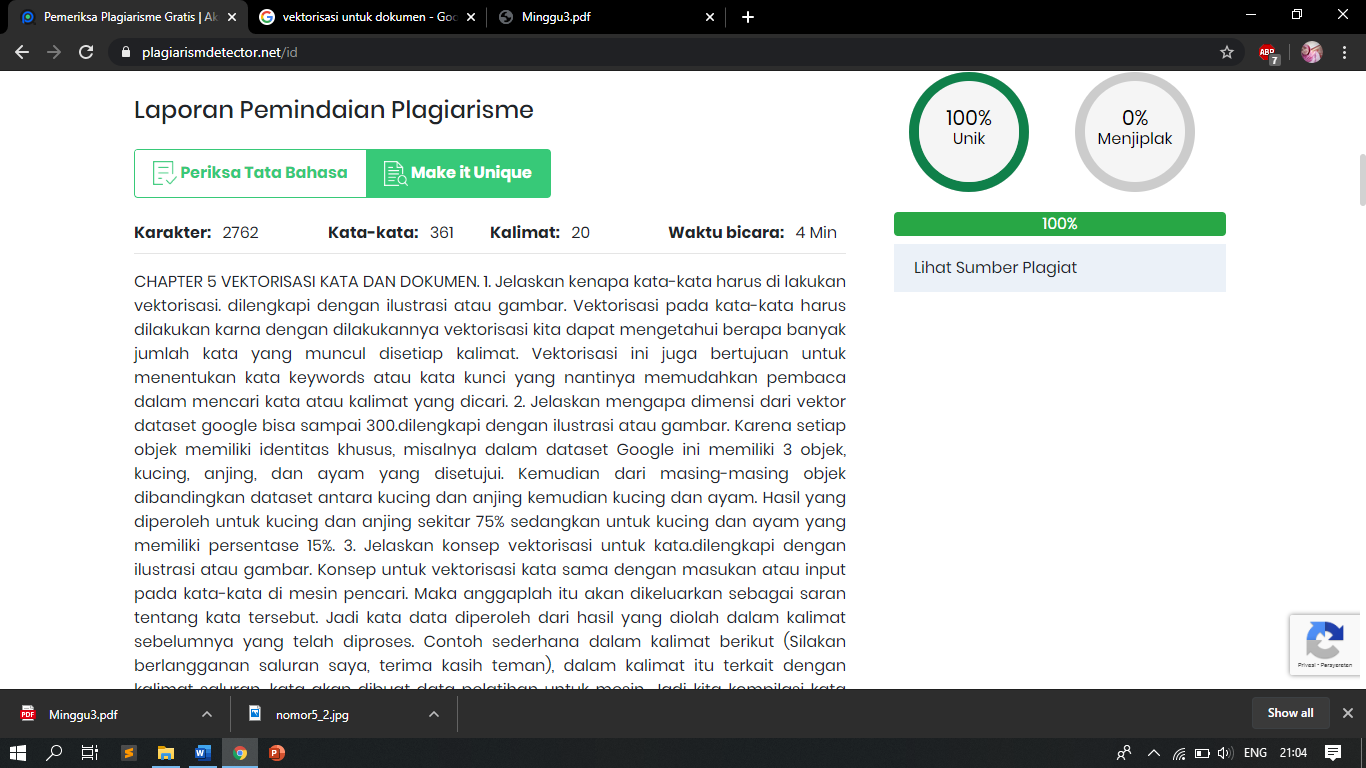
\includegraphics[width=4cm]{figures/1174062/5/tidakplagiat.png}
	\centering
	\caption{Tidak Plagiat}
\end{figure}

